\pgfplotsset{xlabel={\#Unmatched Words / \#Matched Words}}
\pgfplotsset{height=5.5cm,width=8cm}

\resizebox{\textwidth}{!}{%
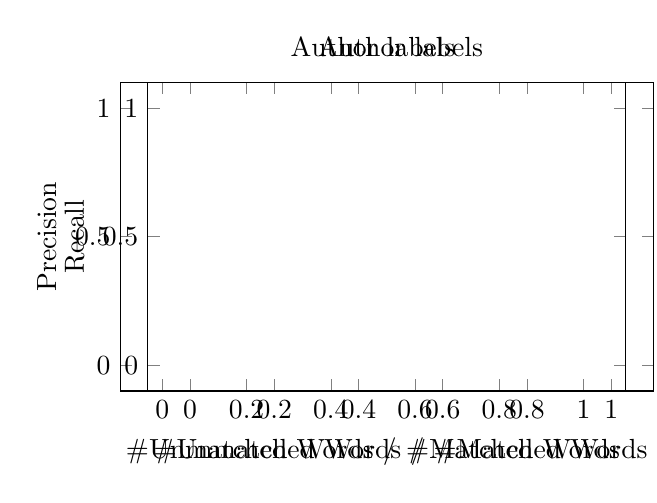
\begin{tikzpicture}
\begin{axis}[
    \firstchartconfig
    title={Author labels},
    ylabel={Precision},
    yticklabel style={/pgf/number format/precision=3},
    \colorlist
]
\plotfile{/home/martin/mt/plots/other-ratios-labels-precision.dat}
\legend{}; % empty the legend
\end{axis}

\hskip 10pt

\begin{axis}[
    \secondchartconfig
    \secondchartlegendconfig
    title={Author labels},
    ylabel={Recall},
    yticklabel style={/pgf/number format/precision=3},
    \colorlist
]
\plotfile{/home/martin/mt/plots/other-ratios-labels-recall.dat}
\end{axis}
\end{tikzpicture}
}

\vspace{10pt}

\resizebox{\textwidth}{!}{%
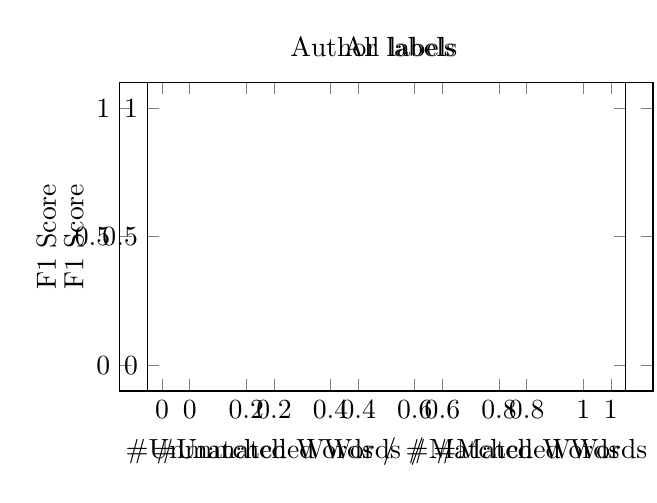
\begin{tikzpicture}
\begin{axis}[
    \firstchartconfig
    title={Author labels},
    ylabel={F1 Score},
    \colorlist
]
\plotfile{/home/martin/mt/plots/other-ratios-labels-f1.dat}
\legend{}; % empty the legend
\end{axis}

\hskip 10pt

\begin{axis}[
    \secondchartconfig
    title={All labels},
    ylabel={F1 Score},
    yticklabel style={/pgf/number format/precision=3},
    legend style={font=\ttfamily},
    \colorlist
]
\plotfile{/home/martin/mt/plots/other-ratios-total-f1.dat}
\legend{}; % empty the legend
\end{axis}
\end{tikzpicture}
}
\vspace*{-\baselineskip}
